\chapter{Калькулятор}

\section{Чем калькулятор отличается от компьютера?}


\section{Калькулятор для 7 операций}

Все вычислители можно соединить с одним и тем же регистром, как хранилищем результата, чтобы получить простейший
калькулятор. Доступны следующие операции:
\begin{enumerate}
    \item Инверсия
    \item Сдвиг вправо
    \item Побитовое И
    \item Побитовое ИЛИ
    \item Исключающее ИЛИ
    \item Сложение
    \item Вычитание
\end{enumerate}

\subsubsection{Практикум}

Список модулей:
\begin{itemize}
    \item Модуль переключателей: $10$ штук
    \item Модуль унарных операций: $2$ штуки
    \item Сумматор: $2$ штуки
    \item Модуль логических операций: $1$ штука
    \item Регистровый модуль как шинный формирователь: $2$ штуки
    \item Регистровый модуль: $1$ штука
    \item Модуль шины: $1$ штука
    \item Соединительные шлейфы: $4$ штуки
\end{itemize}

Уже проверенные модули для разных операций соединяются вместе.
Для этого используются несколько мультиплексоров (шинных формирователей)
на платах регистров. На этих платах не установлены реле для хранения
битов. Вместо этого шины подключаются к одному и тому же регистру.
Так в него можно записывать любой из $7$ результатов вычислений.

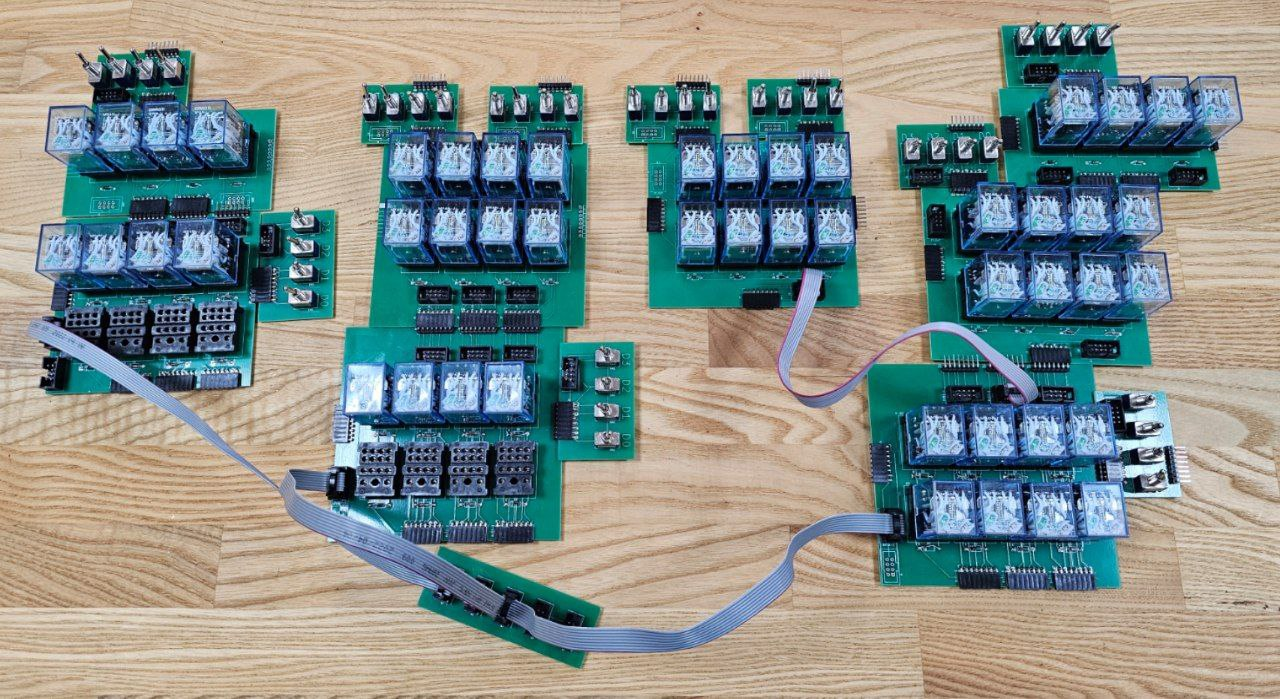
\includegraphics[width=\columnwidth]{photo/calculator.jpg}

Любую из операций можно выполнить так:

\begin{enumerate}
    \item Отключить все управляющие сигналы.
    \item Набрать входные данные для нужной операции.
    \item Подключить выход нужного модуля к регистру тумблером.
    \item Наблюдать результаты вычислений.
    \item Сбросить значение регистра.
\end{enumerate}


\section{Расширение вычислений до восьми бит}

У регистров и вычислительных модулей справа и слева есть разъёмы для расширения разрядности.

Для регистров через эти разъёмы передаются сигналы сброса и подключения к шинам. Поэтому
один набор тумблеров может использоваться для двух четырёхбитных плат-регистров, если они
соединены в один восьмибитный регистр.

Для вычислительных модулей через боковые разъёмы передаются сигналы переноса (в случае сдвига и сложения).

\subsubsection{Практикум}

Соединить два регистра и два сумматора. Шина $3$ регистров подключается к сумматору.
У правого (младшего) сумматора входящий перенос перемычкой устанавливается в $0$.
У левого (старшего) сумматора перемычка для переноса убирается, потому что
сигнал переноса приходит от младших битов (из правого сумматора).

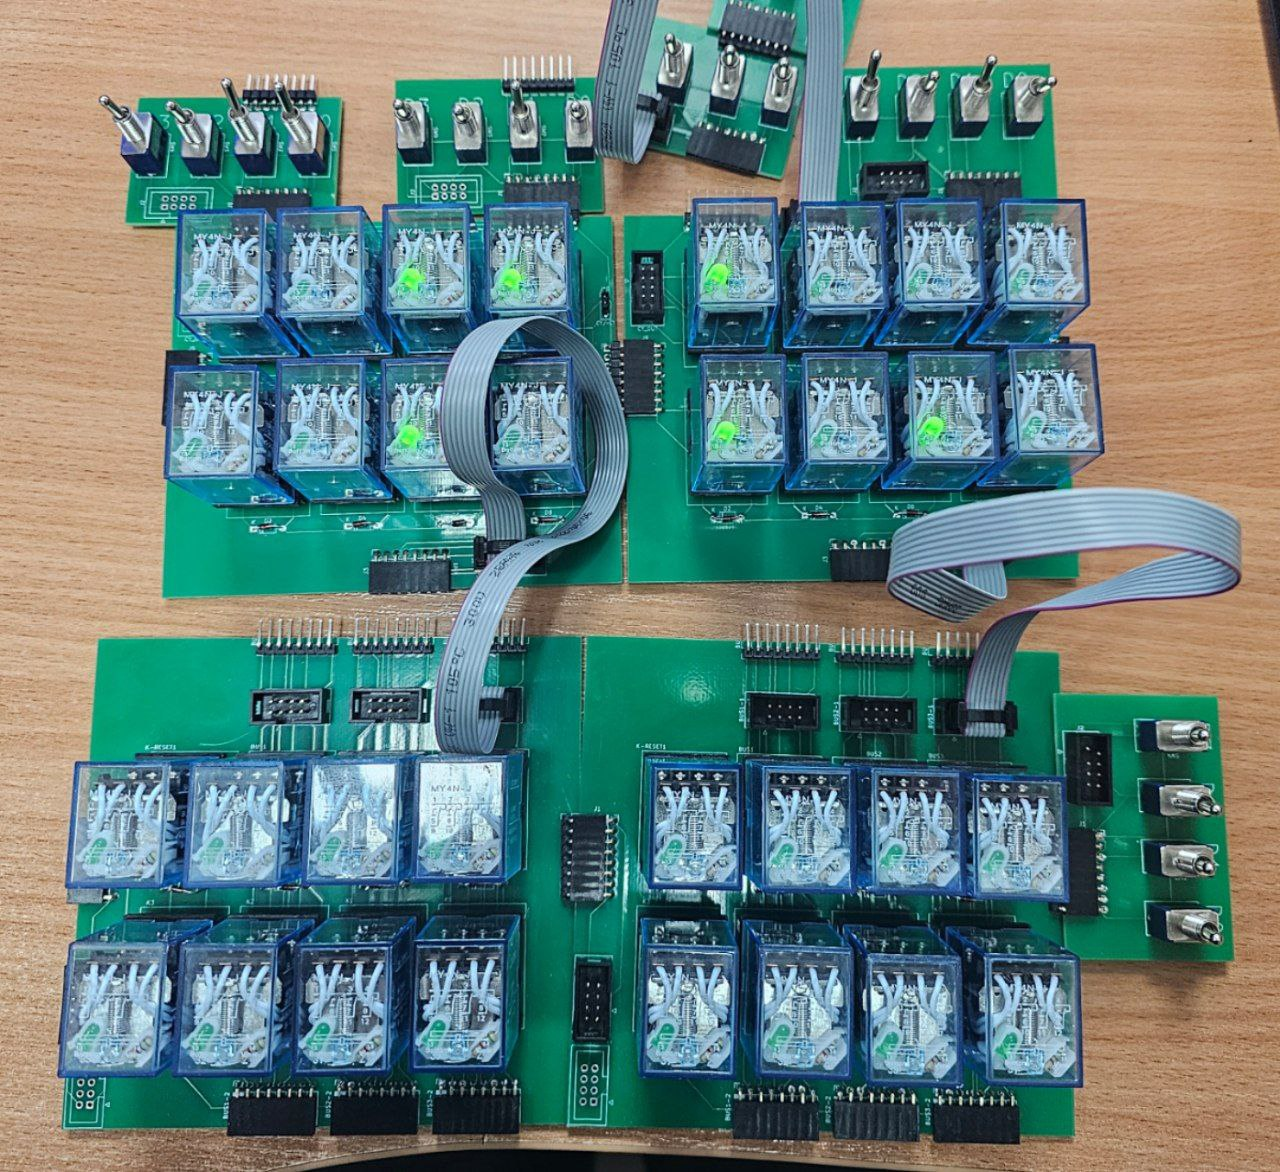
\includegraphics[width=0.5\columnwidth]{photo/8bit.jpg}

\begin{enumerate}
    \item Отключить все управляющие сигналы.
    \item Набрать входные данные $0011 1001$ и $0010 1001$.
    \item Подключить выход сумматора к регистру тумблером $D3$.
    \item Наблюдать результат вычислений $0110 0010$.
\end{enumerate}

